\documentclass[a4paper,12pt]{article}

\usepackage{graphicx}
\usepackage{siunitx}
\usepackage{mathtools}
\usepackage[colorlinks,bookmarks=false,linkcolor=blue,urlcolor=blue]{hyperref}

\baselineskip=16pt
\parindent=15pt
\parskip=5pt

% Custom lengths
\newlength{\plotwidth} % Universal width of Matlab figures
\setlength{\plotwidth}{12cm}

% Custom commands
\def \be {\begin{equation}}
\def \ee {\end{equation}}
\def \dd {{\rm d}}
\newcommand{\mail}[1]{{\href{mailto:#1}{#1}}} % Mail hyperlink
\newcommand{\ftplink}[1]{{\href{ftp://#1}{#1}}}
\newcommand{\abs}[1]{\lvert#1\rvert} % Absolute value
\newcommand{\zM}{z_{Moon}} % Position of the Moon
\newcommand{\mE}{m_{Earth}} % Mass of the Earth
\newcommand{\mM}{m_{Moon}} % Mass of the Moon
\newcommand{\comment}[1]{}

\begin{document}

\title{From the Earth to the Moon}
\author{Lucien Huber, Aman Berdyev \\
{\small \mail{lucien.huber@epfl.ch} , \mail{aman.berdyev@epfl.ch}}}
\date{\today}
\maketitle

\section{Introduction}

In this exercise we were tasked with simulating the path of a bullet/rocket from the famous book \emph{De la Terre \`a la Lune} by Jules Verne. The projectile leaves the earth with an initial velocity $v_0$ and goes in a straight line towards the Moon.


\section{Analytical Computations}

\subsection{Differential equations}

To tackle this problem the axes and origin (at the center of the earth)  are positioned and then the different forces acting upon the projectile are considered:
\be
    m\vec{a} =\sum \vec{F}_{ext} =   \vec{F}_{moon-bullet} + \vec{F}_{earth-bullet}  + \vec{F}_t
\ee
Projecting on the z axis gives:
\be
 m\Ddot{z} = \frac{-z G\mE m}{\abs{z}^3} + \frac{(\zM-z)G\mM m}{\abs{\zM-z}^3} - \frac{\Dot{z}^3\rho S C_x }{ 2\abs{\Dot{z}}}
\ee
Thus the two differential equations obtained are:
\be
\begin{dcases}
    \frac{\dd z(t)}{\dd t}  = v(t) \\
    \frac{\dd v(t)}{\dd t}  = \frac{-z(t) G\mE}{\abs{z(t)}^3} + \frac{(\zM-z(t))G\mM}{\abs{\zM-z(t)}^3} - \frac{v(t)^3\rho S C_x }{ 2\abs{v(t)}}
    \label{eq:diffzv}
\end{dcases}
\ee

\subsection{Equilibrium state}
This section will address the existence of an equilibrium state on the $z$ axis, such that the sum of the gravitational fields of the Earth and the Moon is null. One such equilibrium state \( \vec{z}_E = (0, 0, z_E) \) is expected between the two bodies \( (z_{Earth} < z_E < \zM) \).

The equilibrium state satisfies
\be
    \vec{g}_{Earth}(\vec{z}_E) + \vec{g}_{Moon}(\vec{z}_E) = 0
\ee
where $\vec{g}_{Earth}$ and $\vec{g}_{Moon}$ are the gravitational fields of the Earth and the Moon, respectively.\\
The projection on the $z$ axis gives
\be
    \frac{-z_E G\mE}{\abs{z_E}^3} + \frac{(\zM-z_E)G\mM}{\abs{\zM-z_E}^3} = 0
\ee
The condition \( z_{Earth} = 0 < z_E < \zM \) gives
\begin{gather}
    -\frac{G\mE}{z_E^2} + \frac{G\mM}{(\zM-z_E)^2} = 0 \\
    (\mE-\mM)z_E^2 - (2\mE\zM)z_E + \mE\zM^2 = 0
\end{gather}
The two solutions are of the form
\be
    z_{E_{1,2}} = \zM\left(\frac{\mE\pm\sqrt{\mE\mM}}{\mE-\mM}\right)
\ee
Only the solution that satisfies $z_E < \zM$ is kept
\be
    z_E = \zM\left(\frac{\mE-\sqrt{\mE\mM}}{\mE-\mM}\right)
\ee

Thus, $(0, 0, z_E)$ is the only equilibrium state on the $z$ axis situated between the Earth and the Moon. With the reference values given in the file \verb|configuration.in| $z_E = \SI{3.4603e08}{\meter}$.

\subsection{Initial velocity to reach $z_E$}

The numerical simulations will not faithfully replicate the voyage described by Jules Verne. Instead, the focus is set on launching the bullet from the surface to the equilibrium state described above. The initial velocity $v_0$ will be computed analytically, so that the bullet reaches $z_E$ at zero speed under the hypothesis that the air drag can be ignored $(\rho_0 = 0)$. 

The forces of gravity of both the Earth and the Moon are conservative, with the potentials
\begin{align}
    U_{Earth}(z) &= -\frac{G\mE m}{\abs{z}} \\
    U_{Moon}(z) &= -\frac{G\mM m}{\abs{z-\zM}}
\end{align}
Therefore, the mechanical energy of the bullet is conserved:
\begin{align}
    \frac{m v_0^2}{2} + U_{Earth}(z_0) + U_{Moon}(z_0) &= U_{Earth}(z_E) + U_{Moon}(z_E) \\
    \frac{m v_0^2}{2} - \frac{G\mE m}{z_0} - \frac{G\mM m}{\zM -z_0} &=  -\frac{G\mE m}{z_E} - \frac{G\mM m}{\zM - z_E}
\end{align}
Solving for $v_0 $ gives:
\be
    v_0 = \sqrt{2G\left(\mE\left(\frac{1}{z_0}-\frac{1}{z_E}\right) + \mM\left(\frac{1}{z_E-\zM}-\frac{1}{z_0-\zM}\right)\right)}
\ee
With the reference values this gives: $v_0 = \SI{1.1066e04}{\meter\per\second}$

\section{Numerical simulations}

Two types of simulations will be conducted. The first simulation takes place over a span of 24 hours and does not take the air drag into account. The second one looks more closely at the movement of the bullet through the atmosphere during 10 seconds. Both of them use the system~\eqref{eq:diffzv} to determine the acceleration and then compute the velocity and position by iterating the Euler method:
\begin{align}
    a(t) &= \sum F_z\bigl(z(t),v(t)\bigr)/m \\
    v(t+\Delta t) &= v(t) + a(t)\cdot\Delta t \\
    z(t+\Delta t) &= z(t) + v(t)\cdot\Delta t
\end{align}

\subsection{Simulation without air drag $(\rho_0 = 0)$}

The simulation conducted was done over 86400s. It was repeated 6 times with 1000, 2000, 4000, 8000, 16000, 32000 iterations. The graphs (Fig.~\ref{fig:za(dt)},~\ref{fig:va(dt)}) plot the final position and final velocity with respect to $\Delta t$. By observing both graphs the linear convergence of Euler's method becomes clear as the points plotted form a straight line.

\begin{figure}[p]
    \centering
    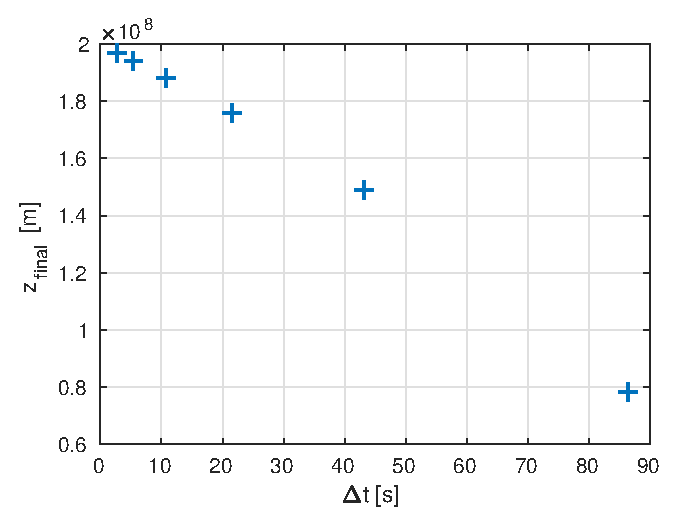
\includegraphics[width=\plotwidth]{ConvergenceZa}
    \caption{Position of the bullet relative to the time step length with no drag}
    \label{fig:za(dt)}
\end{figure}
\begin{figure}[p]
    \centering
    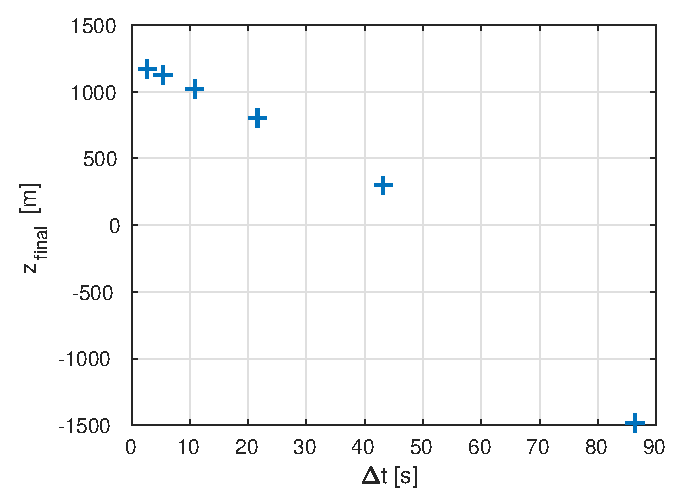
\includegraphics[width=\plotwidth]{ConvergenceVa}
    \caption{Velocity of the bullet relative to the time step length with no drag}
    \label{fig:va(dt)}
\end{figure}

\subsection{Simulation with air drag $(\rho_0 = \SI{1,3}{\kilo\gram\per\cubic\meter})$}
The simulation conducted was done over 10s. It was repeated 6 times with 200, 400, 800, 1600, 3200, 6400 iterations. The graphs (Fig.~\ref{fig:zb(dt)},~\ref{fig:vb(dt)}) plot the final position and final velocity with respect to $\Delta t$. Both graphs confirm the linear convergence of Euler's method.

\begin{figure}[p]
    \centering
    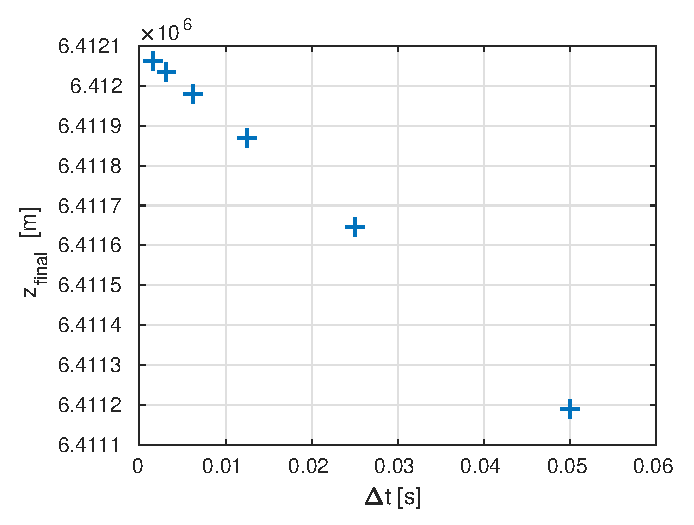
\includegraphics[width=\plotwidth]{ConvergenceZb}
    \caption{Position of the bullet relative to the time step length with drag}
    \label{fig:zb(dt)}
\end{figure}
\begin{figure}[p]
    \centering
    \includegraphics[width=\plotwidth]{ConvergenceVb}
    \caption{Velocity of the bullet relative to the time step length with drag}
    \label{fig:vb(dt)}
\end{figure}

\end{document}
